\documentclass{article}
\usepackage[margin=0.5cm]{geometry}
\usepackage[utf8]{inputenc}
\usepackage{graphicx}
\usepackage{listings}
\usepackage{color}
\usepackage{placeins}
\usepackage{hyperref}
\usepackage{xcolor}
\usepackage{caption}
\usepackage{amsfonts}
\usepackage{amsmath}

\begin{document}

\include{frontpage}

\section*{Relations and Partial-Orders:}
Signature:
$$ :) \subseteq S \times S$$
Members of the relation:\\
$
\{
(\emptyset,\emptyset), 
(\emptyset, \{x+1\}),
(\emptyset, \{2*y\}), 
(\emptyset, \{z/3\}), 
(\emptyset, \{x+1, 2*y\}), 
(\emptyset, \{x+1, z/3\}), 
(\emptyset, \{2*y, z/3\}), 
(\emptyset, \{x+1, 2*y, z/3\}),
%%
(\{x+1\}, \{x+1\}), 
(\{x+1\}, \{x+1, 2*y\}), 
(\{x+1\}, \{x+1, z/3\}), 
(\{x+1\}, \{x+1, 2*y, z/3\}),
%%
(\{2*y\}, \{2*y\}),
(\{2*y\}, \{x+1, 2*y\}),
(\{2*y\}, \{2*y, z/3\}), 
(\{2*y\}, \{x+1, 2*y, z/3\}),
%%
(\{z/3\}, \{z/3\}),
(\{z/3\}, \{x+1, z/3\}), 
(\{z/3\}, \{2*y, z/3\}),   
(\{z/3\}, \{x+1, 2*y, z/3\}),
%%
(\{x+1, 2*y\}, \{x+1, 2*y\}),  
(\{x+1, 2*y\}, \{x+1, 2*y, z/3\}),
%%
(\{2*y, z/3\}, \{2*y, z/3\}),  
(\{2*y, z/3\}, \{x+1, 2*y, z/3\}),
%%
(\{x+1, z/3\}, \{x+1, z/3\}),  
(\{x+1, z/3\}, \{x+1, 2*y, z/3\}),
%%
(\{x+1, 2*y, z/3\}, \{x+1, 2*y, z/3\})
\}$
\vspace{0.5cm}\\
\noindent An example of a member of the relation:\\
$$(\{x+1, z/3\}, \{x+1, z/3\}) \in :)$$
$$\{x+1, z/3\}:)\{x+1, z/3\}$$
An example of a non-member of the relation:\\
$$(\{x+1, z/3\}, \{x+1, z/3\}) \notin :)$$
$$\{x+1, z/3\}\not:)\{x+1, z/3\}$$
Do the set S and relation $:)$ form a partial-order? Yes, because The relation is:\\
\begin{itemize}
	\item Reflexive, every element is related to itself.
	\item Antisymmetric, two elements must not be related in both directions (unless they are the same element).
	\item Transitive, if the first element is related to the second element, and the second is related to the third, then the first is related to the third.
\end{itemize}
Draw a Hasse diagram:\\
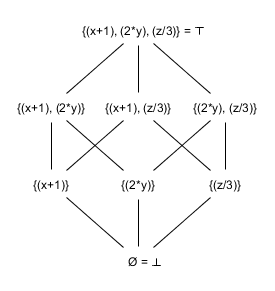
\includegraphics[width=0.5\textwidth]{Hasse}
\pagebreak
\section*{Greatest-Lower-Bound:}
A lower bound $x$ for a set $S$ is defined as:
$$\forall s \in S:\;s \sqsupseteq x$$
If we want to define the greatest lower bound the following must hold:
$$S\sqsupseteq x \land \forall y:\;S\sqsupseteq y \implies x \sqsupseteq y$$
Given a lattice $L = (S, \sqsubseteq)$; what do the elements $\sqcup S$ and $\sqcap S$ correspond to? Assuming $S$ from above, $\sqcap S$ is $\{x+1, 2*y, z/3\}\}$, and $\sqcup S$ is $\emptyset$
\section*{Lattices:}
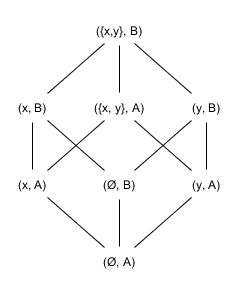
\includegraphics[width=0.5\textwidth]{Lattices}

\noindent A $L_1 \times L_2$ lattice will have $|L_1| * |L_2|$ points. So the resulting lattice will in this case have $2 * 4 = 8$ points.

\end{document}